\chapter{Conventional tide prediction and seamless forecasts}

%-----------------------------------------------
\section{Seamless prediction requires operational signal clarity}

Evolving and improving forecast and observational capabilities.

Idea of seamless and targeted forecasts will rely on hybrids and system aggregation. 


\subsection{OLD text}
Growing sophistication and availability of physical forecast models that address coastal sea level. 
Despite this, we suspect a continuing role for hybrid and aggregation forecasts.


Statistical tidal forecasts continue to robustly offer skill at key locations - especially for routine and long window forecasts.
Targeted physical model configs are successful: eg spectral waves, non-tidal DA mesoscale.

Given this situation, should we specially prepare harmonic tide predictions for aggregation with OGCM?
How much 'nontidal' energy overlaps with or projects onto harmonic analysis - and does it matter?

\begin{itemize}
  \item Determine best method for aggregate sea level, prepare for future changes to NTC, oceanmaps, ACCESS
  \item clairfy and evaluated the significance of overlap, what is in the OGCM?, role of DA and RADS config
  \item open way to future work on: tidal analysis quality of fit and overfit, tide gauges for DA
\end{itemize}


\subsection{ Historical division of prediction }
TBC


\subsection{ Limits to data transparency in operational setting }

(1) Lack of hindcast or re-analysis for every model update.
(2) Lack of availablity of observational record or inhomogeneous inputs to harmonic predictions (eg inferred constiuents or other behind the scenes techniques of conventional tide prediction).

Note exclusion of some potential approaches:
- real time continuious updating tidal ( eg using wavelets )
- other statistical approaches such as multi-input admittance and machine learning methods 
- of even lookup via climate index (ENSO, IOD etc)

In this case we do have  access to 'official' tidal analysis results over ~19 years.  
Very indirect reflection of actual observations, and inclusive of all the inhomogenous pragmatism of tidal centre human intervention and processes.


Tide data via API.



%---------
\subsection{Tide data micro-services}

Forecast applications will increasingly rely on a `microservice` architecture (REF Boston).

Australian tide predictions are ripe for a move to microservice model - but would benefit from differentiation into variants with clear signal intention.

%---------
\subsection{Standard ports, secondary ports and the sausage factory}

National service has evolved to cover a diverse range of community and business requirements.

ANTT split of 'quality' into standard and secondary ports.

In reality many users accustomed to treating all as best effort predictions of mixed quality.

Thriving and evolving service sector via apps (eg AnyTide, etc).
But 'official' predictions maintain special status for a variety of reasons that go well beyond skill assessments:
Eg
\begin{itemize}
    \item wide public trust 
    \item legal requirements for ANTT and navigation
    \item implied liability path 
    \item consistency with government services like warnings etc
\end{itemize}




%---------
\subsection{Apriori distinction of tidal elevation flavours}
At least the following:
\begin{itemize}
    \item standard annual prediction
    \item historical tidal analysis
    \item gravitation ocean tide estimate
    \item datum clarity
\end{itemize}

Such distinctions are not new per se, but the overlap and standarisation into operational environment is?:
\citep{godin:1972}

%-----------------------------------------------
\section{Insitu and spatial tide predictions}

Apriori differences and practical differences.

\begin{itemize}
    \item long periods
    \item shallow water
    \item radiational
\end{itemize}

Cite some typical applications
\begin{itemize}
    \item GA inter-tidal zone mapping activity (TPXO raw)
    \item CSIRO currents (TXPO as OBC)
    \item Bluelink downscales (TBC)
    \item BoM downscales (TBC)
    \item UWA (TBC)?
\end{itemize}

%---------
\subsection{How do global tide solutions differ from local insitu predictions}
TBC

\subsection{resolution versus risk of category-error}
Is it all about coastal bathymetry resolution?

Not only that.

Fit-for-purpose.

Assertions about tidal constants - persistence of a fixed admittance.   Let alone physical coverage of the admittance.


%---------
\subsection{TPXO versus BoM (versus CSIRO)}
Timeseries stats at locations.

Aims and inclusions.
\begin{itemize}
    \item pick time period to match csiro
    \item lookup tides full
    \item lookup tides no radiational
    \item otps to match points
    \item csiro (opendap) pick points and map to llookup tides file
    \item RMSE/Bias ...maybe Taylor
\end{itemize}

Analysis:
* significance of long periods

Comments on rejected by CSIRO.

%---------
\subsection{Addition: relevance to TWL forecasts}
Tides as OBC to local models.

Tides as superposition component.

%---------
\subsection{Relevance to assimilation of SLA}
Altimetery uses global solution.

Implications for use of tide gauges for DA.


%-----------------------------------------------
\section{Current state of 'official' predictions}

National service, ANTT, navigation and survey.

%---------
\subsection{How constant are 'official' predictions}

Note intention and operational stetting

* evolution of ZFL
plot


\begin{figure}[h]\centering
  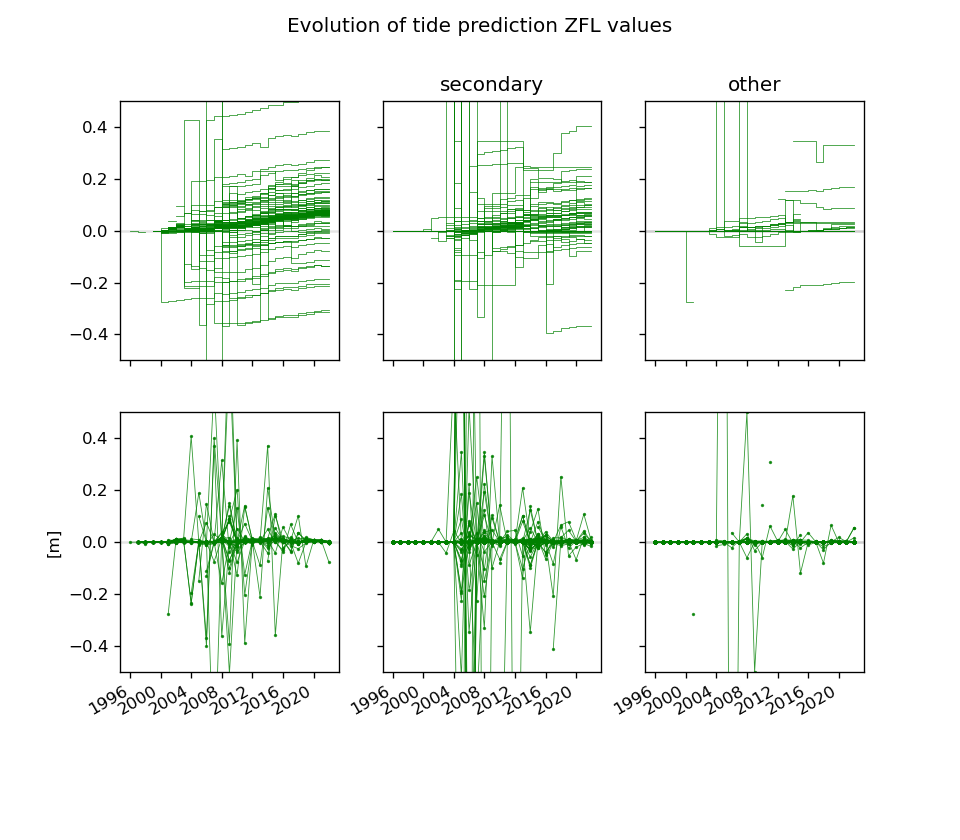
\includegraphics[width=150mm]{figures/plots/tidal_z0_evolution.png}
  \caption{Historical evolution of zero frequency level in Australian tide predictions}
  \label{fig:tbc}
\end{figure}

%---------
\subsection{mean sea level and long periods}

Ref to MHL compare.

\subsubsection{length and quality of training data}

Well known - but easily dropped in downstream applications.
Best efforts.


%-----------------------------------------------
\section{Tidal projection applied to nontidal forecasts}
%---------
\subsection{oceanmaps + aggregated}
TBC

%---------
\subsection{access-s and or BRAN}
TBC



no surprise
premise of harmonic analysis - only identify stable.
useful in so far as it is stable.

foreman analysis - allows for some measure of matrix condition (though Gaussian)


\subsection{ recent forecasts }
verify files


\subsection{ long free run climate model }
cosima
no DA shocks
dailys only


%-----------------------------------------------
\section{Proposed differentiation of operational tide services}
\subsection{Conventional prediction service ANTT}

TBC

\subsection{Standard navigation ANTT}

TBC
